\documentclass{article}

\usepackage{graphicx}
\usepackage{subfigure}

\begin{document}

\section{Inhalation}
\subsection{Control Circuit}
\begin{figure}[h]
\centering
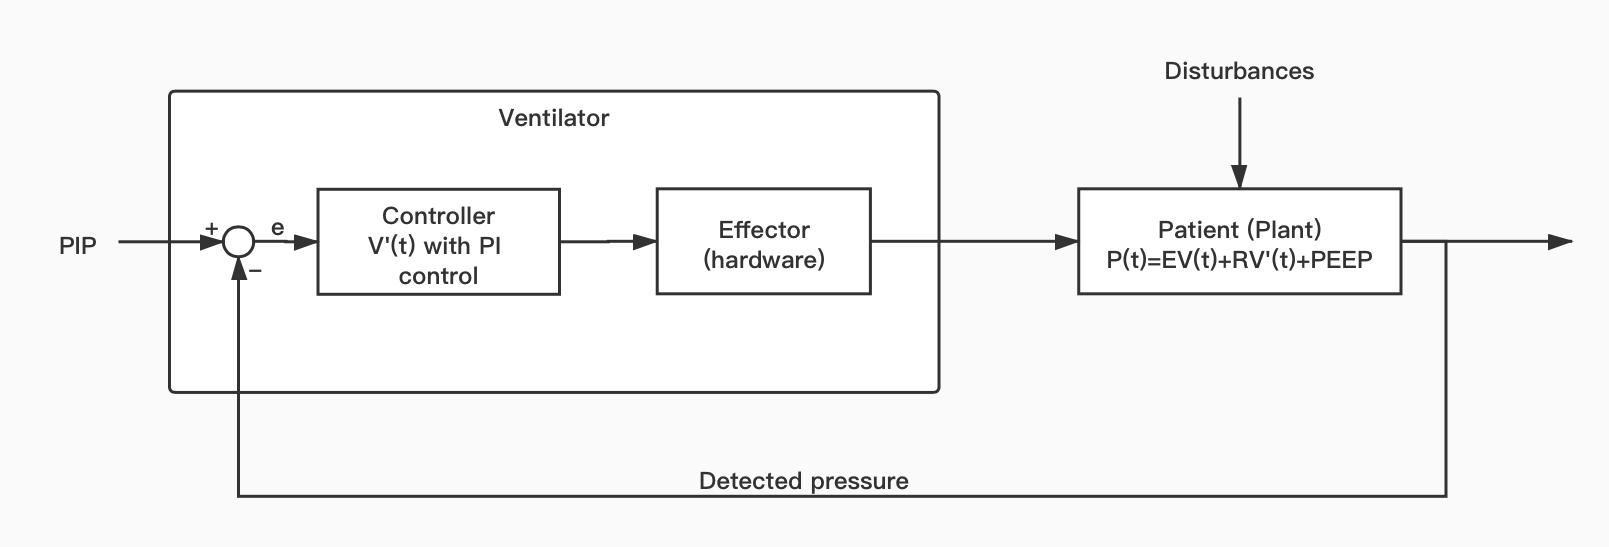
\includegraphics[scale=0.23]{control-circuit.jpg}
\end{figure}

The control circuit for inhalation. The input $PIP$ (Peak Inspiratory Pressure) is the expected level of pressure to reach. Error $e$ is the difference between actual pressure $P(t)$ measured by the sensor and $PIP$. $V(t)$ is the volume of air in patient's alveoli and $V'(t)$ would represent the flow speed of the injected gas. PI control is used in the circuit. The formula for the controller is :
$$V'(t)=K_pe+K_i\int _0^tedt$$
For the plant, the formula
$$P(t)=EV(t)+RV'(t)+PEEP$$
is the equation of motion, which shows a mathematical relation between the physical properties in the patient's lung. $E$ represents the elastance (inverse of the compliance) of the patient's lung and $R$ represents the airway resistance. $PEEP$ (Positive End Expiratory Pressure) is the remaining positive pressure in the patient's lung after exhalation. It is usually set as positive manually to prevent atelectasis.

\newpage

\subsection{Flow Diagram}
\begin{figure}[h]
\centering
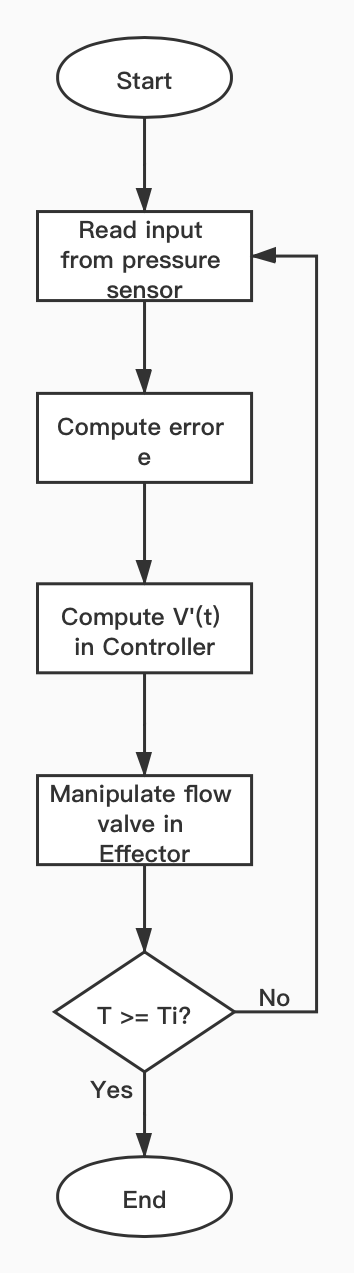
\includegraphics[scale=0.3]{flow-diagram.jpg}
\end{figure}

The flow diagram for a single inhalation. It can be triggered either by the machine or by patient. When the time $T$ has exceed the preset inspiratory time $Ti$, the inhalation would end and the exhalation would begin.

\newpage

\subsection{Transfer Function}
\begin{figure}[h]
\centering
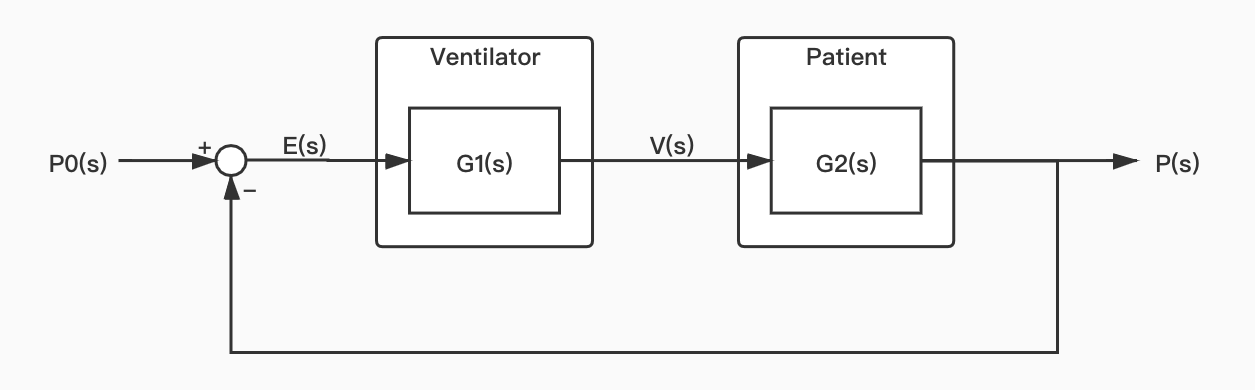
\includegraphics[scale=0.3]{block-diagram.jpg}
\end{figure}

$E(s)$, $V(s)$, $P(s)$ is the Laplace transforms of the error $e(t)$, volume $v(t)$ and the pressure $p(t)$. The input $P_{0}(s)$ is the Laplace transform of $p_{0}$, while $p_{0}$ is $PIP-PEEP$. $PEEP$ is subtracted from $PIP$ so that the zero initial condition of the system can be satisfied ($p(0)=0$). $G_1(s)$ is the transfer function of the ventilator and $G_2(s)$ is the transfer function of the patient.

For ventilator:
$$v'(t)=K_pe+K_i\int _0^tedt$$
Do Laplace transform on both sides:
$$sV(s)=K_pE(s)+\frac{K_i}{s}E(s)$$
$$G_1(s)=\frac{V(s)}{E(s)}=\frac{K_p}{s}+\frac{K_i}{s^2}$$

For patient:
$$p(t)=Ev(t)+Rv'(t)$$
Do Laplace transform on both sides:
$$P(s)=EV(s)+RsV(s)$$
$$G_2(s)=\frac{P(s)}{V(s)}=E+Rs$$
$$G(s)=\frac{P(s)}{E(s)}=G_1(s)\cdot G_2(s)=(\frac{K_p}{s}+\frac{K_i}{s^2})(E+Rs)$$
$$P(s)=G(s)\cdot E(s)=G(s)\cdot (P_0(s)-P(s))$$
$$\frac{P(s)}{P_0(s)}=\frac{G(s)}{1+G(s)}$$
Therefore, the transfer function of the system is:
$$\frac{P(s)}{P_0(s)}=\frac{G(s)}{1+G(s)}=\frac{(sK_p+K_i)(E+Rs)}{s^2+(sK_p+K_i)(E+Rs)}$$

\section{Exhalation}
Constructing

\end{document}